\documentclass[titlepage]{article}
\usepackage[utf8]{inputenc}
\usepackage{graphicx}
\usepackage[usenames,dvipsnames,svgnames,table]{xcolor}
\usepackage{fancyvrb}

\title{NanoLab Server}
\author{Joel Johnson }
\date{2017}

\begin{document}

\maketitle

\tableofcontents
\newpage\listoffigures

\newpage\section{Introduction}

    NanoLab is a locally hosted, ultra-secure, and globally accessible large data hosting server for Dr. John Gibbs' Nanophysics Research Laboratory at Northern Arizona University. It has a current storage capacity of ten terabytes, with the ability to expand max capacity in the future as needed, and is running on a Linux-Apache-MySQL-PHP (LAMP) server architecture. NanoLab can be thought of as being composed of two parts: the back-end and the front-end. The back-end is where the actual file storage and handling takes place. This is accomplished with the LAMP server stack software mentioned earlier interacting with the physical hardware of the server box itself. The front end is what the user sees via the web interface in the browser. The web interface is designed, organized, and stylized to create a more user-friendly point of access to the data stored in the back-end, as well as to allow access from anywhere in the world simply through one's browser. The front-end web interface utilizes the standard suite of web development languages$-$HTML, CSS, and JavaScript$-$along with PHP to bridge the front-end and the back-end.
    
    The goal of this document is to provide an administrator-level user guide for when I leave and am no longer able to actively manage the system. There should be very little to do, and what does need to be done will need to be done very infrequently. This document is structured as follows. First, I will describe the physical hardware that comprises NanoLab, as well as outline recommended upgrades that might be desired or necessary in the future. Next, I will briefly discuss the back-end of the server inasmuch as is strictly necessary for proper knowledge and management of the system. Third, I will document the front-end web interface. This front-end section will be more exhaustive than is necessary for an administrator to know, but since it is my original work and it is where the large majority of my time was spent, I will record in detail the inner workings of the web interface. Next I will describe periodic maintenance that must be performed to NanoLab. I also provide a few hardware upgrade options for if the occasion arises when NanoLab is no longer able to meet the needs of the lab. Next I dedicate a chapter as a quick reference guide that contains all the commands that are necessary for managing the system, as well as perhaps some that are not strictly necessary but would make the new administrator's life easier. Following the quick reference guide is a chapter on light troubleshooting steps in the event that something goes wrong. What will be provided here in the way of troubleshooting, however, is not expected to be a comprehensive treatment of any issue. I will be happy to respond to questions, issues, or requests, and generally be as helpful as I am able to be after I leave. My contact information is provided at the end of the document.
    
\section{Physical Hardware}

    The range of hardware that is used for servers is as wide as the range of purpose for all the different types of servers. A server can be as elaborate as a warehouse full of rack-mounted hardware costing millions of dollars, but it can also be as simple as an old laptop. The decision for what is needed is based mostly on how many people will be demanding the server's resources simultaneously and the magnitude of the server's resources each person will be demanding; basically how often and how hard will the server be hit. 
    
    For Dr. Gibbs' research lab, this was an easy question to answer: compared to the massive industrial scale servers, not very often and not very hard. Thus, the server could be built into an older and unused computer that was being stored in the lab. This could easily service the ~10-15 individuals that would be uploading and downloading files from the server, and provided the file sizes aren't too large it could service everyone simultaneously. The biggest limiting factor in the build is the amount of memory. The maximum amount of memory that the motherboard can support is only 8GB. This would be fine for ordinary tasks of a personal computer, but servers utilize ram in a much more intensive way than PC's do. Specifically, the server first needs to place any file being uploaded entirely into ram, so the 8GB of ram severely limits the maximum file size that can be uploaded. The best solution to this without upgrading to better hardware is to compress uploads by zipping files.
    
    \begin{figure}[t]
    \centering
    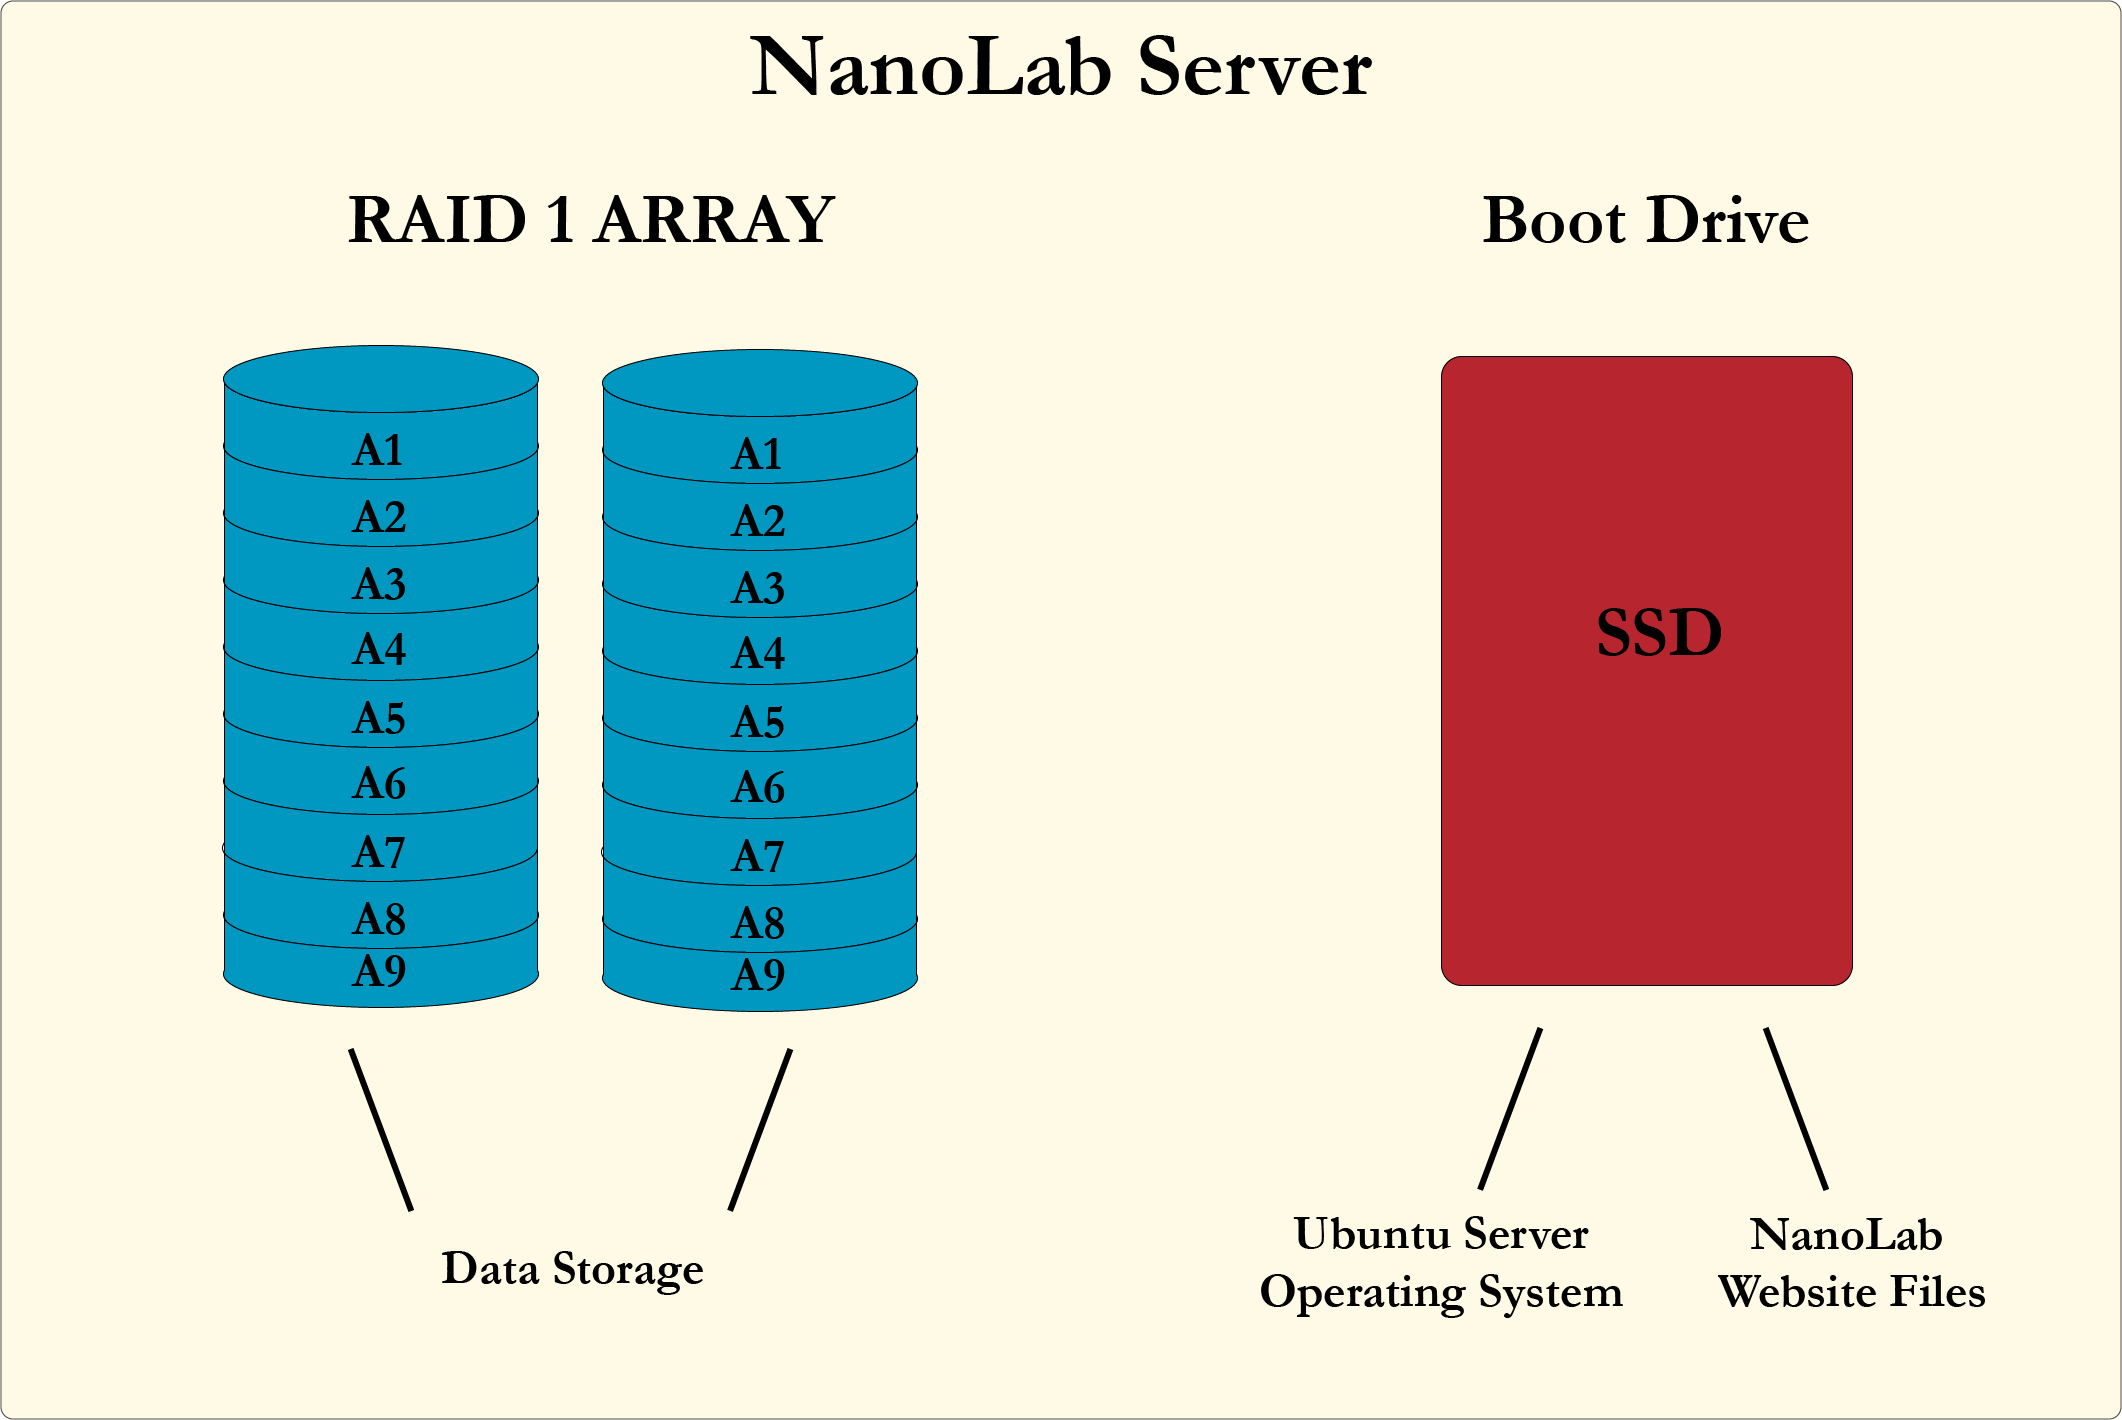
\includegraphics[width=120mm]{Architecture.png}
     \caption{Diagram of Drive Architecture of NanoLab Server}
     \medskip
     \small 
     Each drive is an exact mirror copy of the other drive. In a RAID 1 configuration, any one drive can fail without any loss of data.
     \label{Architecture}
    \end{figure}
    
    The entirety of the specific hardware of this computer isn't entirely pertinent to know, but just for reference's sake here it is listed:
    
    \begin{itemize}
    \item CPU: 
    \item Motherboard: Dell
    \item RAM: 8GB ECC DDR2
    \item SSD: 120GB Samsung 850 Evo
    \item HDD: x2 10TB Western Digital Red
    \item PSU: 850W EVGA T2 Supernova
    \item UPS: 850 VA CyberPower Sinewave
    \end{itemize}

    The ECC on the ram stands for Error Correcting Code. This type of memory is highly desired when mistakes cannot be tolerated, such as servers and scientific computing. The SSD is used as the boot drive. This is where Ubuntu Server is installed as well as where the website files reside. The two HHDs are obviously where the bulk data is stored. Everything uploaded through the website gets filed away on these two drives. Each drive is a mirror copy of the other, called a RAID 1 configuration (Redundant Array of Inexpensive Disks). See figure \ref{RAID1} for a visualization of a RAID 1 configuration. A possible future upgrade would be to add additional identical HDDs and grow the RAID 1 array into a RAID 5 or RAID 6 array. Another possible future upgrade would be to have an additional blank spare identical HDD, known as a hot spare. More info on these upgrades can be found in the Upgrade Possibilities section of this document.

    \begin{figure}[t]
    \centering
    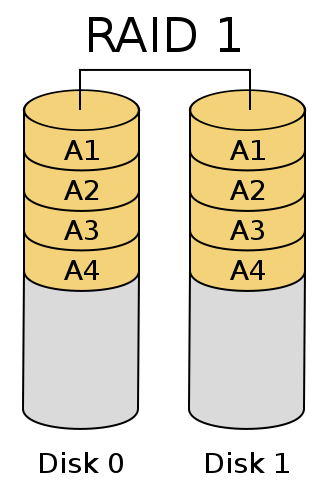
\includegraphics[width=50mm]{RAID1.png}
     \caption{Diagram of a two drive RAID 1 setup}
     \medskip
     \small 
     Each drive is an exact mirror copy of the other drive. In a RAID 1 configuration, any one drive can fail without any loss of data.
     \label{RAID1}
    \end{figure}

\section{Back-End}

    \noindent\textit{Map of drives and data}
    
    NanoLab contains a RAID 1 array of two 8 TB HDDs and one 128 GB SSD (figure \ref{Architecture}). The RAID array is completely dedicated to the actual data needing to be stored by the users and the SSD is used to hold the operating system and all web files needed to host the website. From the root directory, the RAID array is located in:
    
    \begin{verbatim}
        /mnt/Raid1Array
    \end{verbatim}
    
    The data on the RAID array is organized such that the highest level directory is
    
    \begin{verbatim}
        /JohnGibbs
    \end{verbatim}
    
    so that John Gibbs will have the highest level access to all data stored on NanoLab. Within this JohnGibbs directory is a directory for every other user:
    
    \begin{verbatim}
        /JohnGibbs/JoelJohnson
        /JohnGibbs/DylanNicholls
        /JohnGibbs/SamSarker
        ...
    \end{verbatim}
    
    When users, including John GIbbs, log into NanoLab they see the contents of their respective directory. In this way, John Gibbs sees every user's names as directories when he logs in. It is very important to the functionality of the site for all other users that John Gibbs does not change the name of any of the user's name folders. For example,
    \\
    
    {\color{red}
    \noindent do not rename
    \begin{verbatim}
        JohnGibbs/DylanNicholls
    \end{verbatim}
    to 
    \begin{verbatim}
        JohnGibbs/Dylan Nicholls
    \end{verbatim}
    }
    \noindent See figure \ref{DoNotRename} for graphical clarification of this important point.
    \\
    
    \begin{figure}[t]
    \centering
    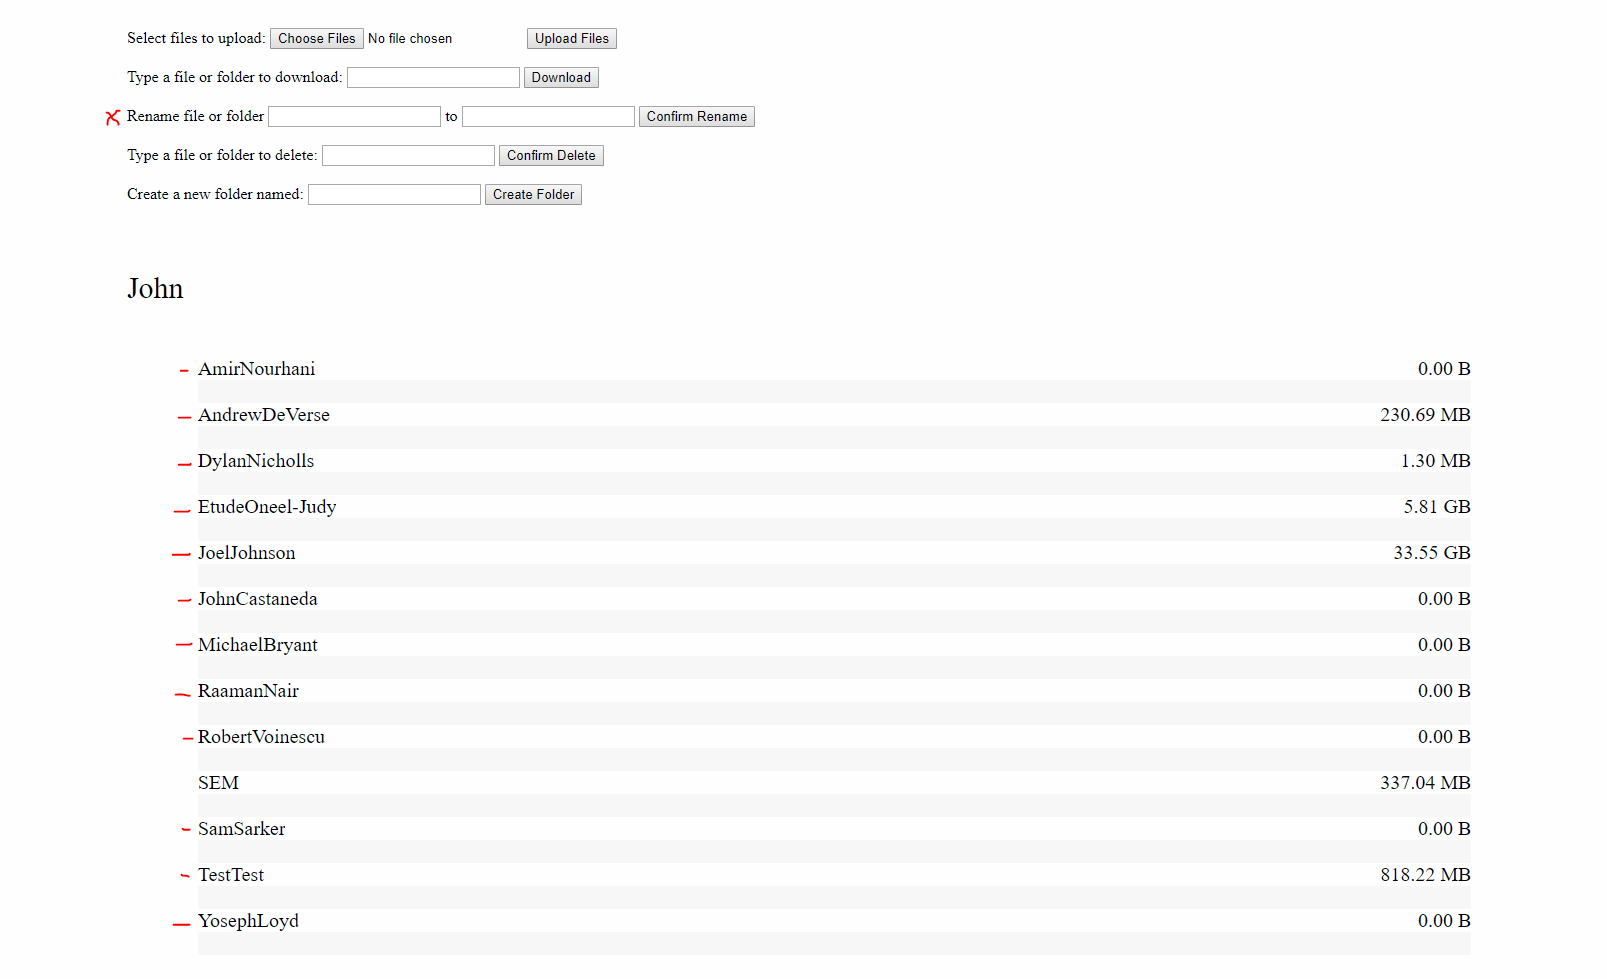
\includegraphics[width=125mm]{DoNotRename.png}
     \caption{Do Not Rename Users Root Folders}
     \medskip
     \small 
     Do not rename any of the folders in the John Gibbs root directory that correspond to other user's root folders.
     \label{DoNotRename}
    \end{figure}
    
    \noindent\textit{PHP Code}
    \\
    
    \noindent\textit{Possibilities for future improvements to platform - RAIS}
    
\section{Front-End}

    HTML, CSS, Javascript 
    \\
    
    \noindent Design
    \\
    
    \noindent Possibilities for future improvements to user interface

\section{Periodic Maintenance}

    \textbf{Ubuntu Server Security Updates}
    
        Just like any operating system, Ubuntu Server periodically has security updates that need to be applied. Of course, the sooner these updates are applied the better and more secure the server is, but it is not critically necessary to check for them every day or even week. In fact, if you are reading this and you realize that years have passed since the last time you checked for updates, don't worry, all is probably fine (but better to take the time to update it now). As a general rule, update Ubuntu Server every 1-3 months. This update schedule would no doubt turn a serious IT professional's hair gray instantly, but we will call it good enough for us.
        
        To check for updates, you only need to log in to the NanoLab terminal (meaning connect a display and keyboard to NanoLab itself and log in using the credentials listed in the Quick Reference Guide section). Upon logging in you will be greeted by the message of the day, within which will be statements about how many updates are ready to be installed.
        
        To apply these updates, type:
        
        \begin{verbatim}
            sudo apt upgrade
        \end{verbatim}
        
        Upon entering this command, Ubuntu Server will download the necessary packages and then confirm with you whether you would still like to install the updates (Y/N), to which you would reply "yes" by typing:
        
        \begin{verbatim}
            Y
        \end{verbatim}
        
        That's it! No further commands are necessary, so you may disconnect the display and keyboard and leave it alone to it's installing if you like. Or you can watch the progress bar as it installs everything and marvel at what a hard day's work you've just done with your server, all the while contemplating when the machines will finally just take over already because they half deserve it.
    \\
    
    \noindent\textbf{Air hose to clean off dust}
    
        This one is rather obvious, but it bares stating that one should be careful not to introduce problems to a perfectly working system by accidentally bumping a cable while cleaning the machine with an air hose, thus causing it to become unplugged just enough to create a spark that kills your entire system upon turning it back on. I'm sure this won't happen to you, however it's never comforting to remember that this very sentiment was shared by everybody whom this has actually happened to. 

\section{Hardware Upgrade Options}

    The following are available hardware upgrades that may be made to NanoLab to accommodate any present or future increase in demand on the hardware.
    \\
    
    \noindent\makebox[\linewidth]{\rule{\textwidth}{0.4pt}}
    \\

    \noindent\textbf{Grow RAID 1 array into a RAID 5 array} with additional identical HDDs
    \\
    
    \noindent\textit{Benefit} $-$ Gain storage space while still maintaining a concurrent fault tolerance of any one drive. This means that any one of the three or more drives can die and no data is lost. See figure \ref{RAID5} for a visualization of a RAID 5 configuration and the Wikipedia page for "Standard RAID Levels" for more info on all RAID configurations.
    \\
    
    \noindent\textit{Estimated Cost} $-$ Current cost of Western Digital Red 10 TB hard drives. RAID 5 requires a minimum of three identical drives.
    \\
    
    \noindent To perform this upgrade or any other upgrade, contact me and I will assist as much as I can in picking out and installing hardware.
    \\
    
    \begin{figure}[t]
    \centering
    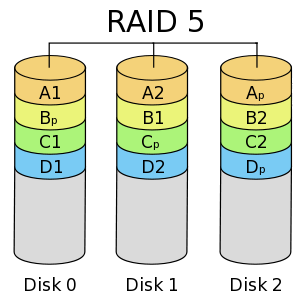
\includegraphics[width=75mm]{RAID5.png}
     \caption{Diagram of a three drive RAID 5 setup}
     \medskip
     \small 
     Each color represents the group of blocks in a respective parity block (a stripe). In RAID 5, parity is distributed equally among each of the drives such that if any one drive fails there is enough remaining data to rebuild the full array.
     \label{RAID5}
    \end{figure}
    
    \noindent\makebox[\linewidth]{\rule{\textwidth}{0.4pt}}
    \\
    
    \noindent\textbf{Grow RAID 1 array into a RAID 6 array} with additional identical HDDs
    \\
    
    \noindent\textit{Benefit} $-$ Gain storage space while maintaining a concurrent fault tolerance of any two drives. This means that any two of the four or more drives can die at the same time and no data is lost. See figure \ref{RAID6} for a visualization of a RAID 6 configuration and the Wikipedia page for "Standard RAID Levels" for more info on all RAID configurations.
    \\
    
    \noindent\textit{Estimated Cost} $-$ Current cost of Western Digital Red 10 TB hard drives. RAID 6 requires a minimum of four identical drives.
    \\
    
    \noindent To perform this upgrade or any other upgrade, contact me and I will assist as much as I can in picking out and installing hardware.
    \\
    
    \begin{figure}[t]
    \centering
    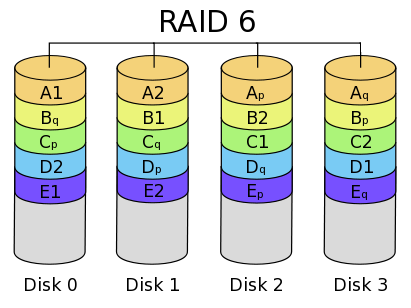
\includegraphics[width=75mm]{RAID6.png}
     \caption{Diagram of a four drive RAID 6 setup}
     \medskip 
     \small 
     Identical to RAID 5 except that RAID 6 extends RAID 5 by adding another parity block. Thus, it uses block-level striping with two parity blocks distributed across all member drives. In this way, even if two drives fail at once there is enough remaining data to rebuild the full array.
     \label{RAID6}
    \end{figure}
    
    \noindent\makebox[\linewidth]{\rule{\textwidth}{0.4pt}}
    \\
    
    \noindent\textbf{Add a hot spare} identical HDD.
    \\
    
    \noindent\textit{Benefit} $-$  A hot spare HDD immediately takes the place of a drive upon failure and starts rebuilding the RAID array with itself. See Wikipedia page for "Hot Spare" for more info on this.
    \\
    
    \noindent\textit{Estimated Cost} $-$ Current cost of Western Digital Red 10TB hard drives. 
    \\
    
    \noindent To perform this upgrade or any other upgrade, contact me and I will assist as much as I can in picking out and installing hardware.
    \\
    
    \noindent\makebox[\linewidth]{\rule{\textwidth}{0.4pt}}
    \\
    
    \noindent\textbf{Modern PC-grade hardware}: motherboard, cpu, and ram
    \\
    
    \noindent\textit{Benefit} $-$ Main benefit would be more memory, which is the biggest limiter with the current setup. Modern PC hardware can provide a serious upgrade without getting into the more pricey terrain of server-grade hardware. At the time of writing, higher-end PC motherboards can support 128 GB of memory for less than the cost of a server-grade Xeon compatible motherboard. Less high-end motherboards still offer more maximum ram capacity than the currently used motherboard (which supports a maximum of 8 GB). At the time of writing, 16 GB is budget, 32 GB standard, and 64 GB is higher-end, and 128 GB is about the maximum.
    \\
    
    \noindent\textit{Estimated Cost} $-$ Completely depends, but with prices at the time of writing, around \$500 - \$600 for 64 GB ram configurations. See pcpartpicker.com/list for more info on hardware configuration compatibility, specs, and current prices.
    \\
    
    \noindent To perform this upgrade or any other upgrade, contact me and I will assist as much as I can in picking out and installing hardware. This upgrade would require a complete physical rebuild of the system (this probably sounds harder than it really is), a re-installation of the operating system, a remounting of the RAID array, and a reloading of NanoLab website files. 
    \\
    
    \noindent\makebox[\linewidth]{\rule{\textwidth}{0.4pt}}
    \\
    
    \noindent\textbf{Server-grade hardware}: the Xeon upgrade
    \\
    
    \noindent\textit{Benefit} $-$ Again, the main benefit would be more memory, but this kind of an upgrade would introduce a myriad of other benefits as well. As for the memory, the sky is the limit with server-grade hardware. You can build a system with a full 1 TB of memory if you have a cool \$13,500 available. Honestly, while this option is certainly available, if you are in a position to actually consider real enterprise-grade server hardware then I am not the guy to talk to. I only include it in this document to provide a ceiling for the upgrades I can help with.
    \\
    
    \noindent\textit{Estimated Cost} $-$ Beyond the scope of my help.
    \\
    
    \noindent\makebox[\linewidth]{\rule{\textwidth}{0.4pt}}
    \\
    
\section{Quick Reference Guide}

    The following bits brief instruction might be useful as a quick reference for periodic interaction with NanoLab on an administrative level.
    \\
    
    \noindent\makebox[\linewidth]{\rule{\textwidth}{0.4pt}}
    \\
    
    \noindent\textbf{NanoLab Terminal Login:}
    
    \begin{verbatim}
        Username: john
        Password: Faraday1791
    \end{verbatim}

    \noindent\makebox[\linewidth]{\rule{\textwidth}{0.4pt}}
    \\

    \noindent\textbf{Update Ubuntu Server for Security Updates:}
    
    \begin{verbatim}
        sudo apt upgrade
    \end{verbatim}

    \noindent\makebox[\linewidth]{\rule{\textwidth}{0.4pt}}
    \\

    \noindent\textbf{Raid array mounted at:} 
    
    \begin{verbatim}
        /mnt/Raid1Array
    \end{verbatim}
    
    \noindent\makebox[\linewidth]{\rule{\textwidth}{0.4pt}}
    \\
    
    \noindent\textbf{Site hosted at:} 
    
    \begin{verbatim}
        /var/www/html
    \end{verbatim}
    
    \noindent\makebox[\linewidth]{\rule{\textwidth}{0.4pt}}
    \\
    
    \noindent\textbf{To check the health of 10 TB drives and the raid array:}
    
    \begin{verbatim}
        sudo mdadm --detail /dev/md0
    \end{verbatim}
    
    \noindent\makebox[\linewidth]{\rule{\textwidth}{0.4pt}}
    \\
    
    \noindent\textbf{To mount a USB stick or any external drive} in order to copy or backup boot drive files or for any other reason, plug in the drive and then type:
    \\
    
    \begin{verbatim}
         lsblk
    \end{verbatim}
    
        Search for your drive in the list of all connected drives (it will most likely be sdd1, but you can confirm which one it is by finding the drive with the capacity that matches your drive). Then type:
    \\
    
    \begin{verbatim}
        sudo mount /dev/sdd1 /mnt/ThumbDrive
    \end{verbatim}

        If your device is listed as something other than sdd1, use that label in place of sdd1 in the code above. Your drive is now mounted, i.e. you can now read and write to the drive. The location of your drive is:
    \\
    
    \begin{verbatim}
        /mnt/ThumbDrive
    \end{verbatim}
    
        To unmount your external drive after you are done (similar to ejecting, but mandatory), you must execute this command:
    \\
      
    \begin{verbatim}
        sudo umount /mnt/ThumbDrive
    \end{verbatim}

        Once the command finishes executing (a couple of seconds), you may remove your drive from NanoLab.
    \\
        
    \noindent\makebox[\linewidth]{\rule{\textwidth}{0.4pt}}
    \\

    Commands for other trivial operations such as copying and moving files can be found online by searching "common unix commands". No copying or altering of files on the boot drive should ever be necessary. As one might expect, altering files on the boot drive may break NanoLab's operating system and/or the website. If this happens don't panic; no critical data is lost in the event of some operating system or website failure. Just contact me (joel@paramag.net or joel.johnson675@gmail.com) and I can assist in rebuilding the system. 

\section{Light Troubleshooting}

    If Nanolab doesn't wake up to show a terminal interface, i.e. it doesn't show anything on the display when you connect a display and keyboard to the physical NanoLab machine, turn NanoLab off and back on again. This shouldn't ever happen, but since it happened to me once it might happen again.
    \\
        
    \noindent\makebox[\linewidth]{\rule{\textwidth}{0.4pt}}
    \\

\section{Contact Information}

    I can be reached in the following ways:
    \\
    
    \noindent\textbf{Email} 
    \\
    
        joel@paramag.net
    
        joel.johnson675@gmail.com
    \\
    
    \noindent\textbf{Phone}  
    \\
    
        916.956.0487

\end{document}
